\documentclass[border=10pt]{standalone}
\usepackage{newtxtext, newtxmath}
\usepackage{tikz}
\usetikzlibrary{bayesnet}

\begin{document}
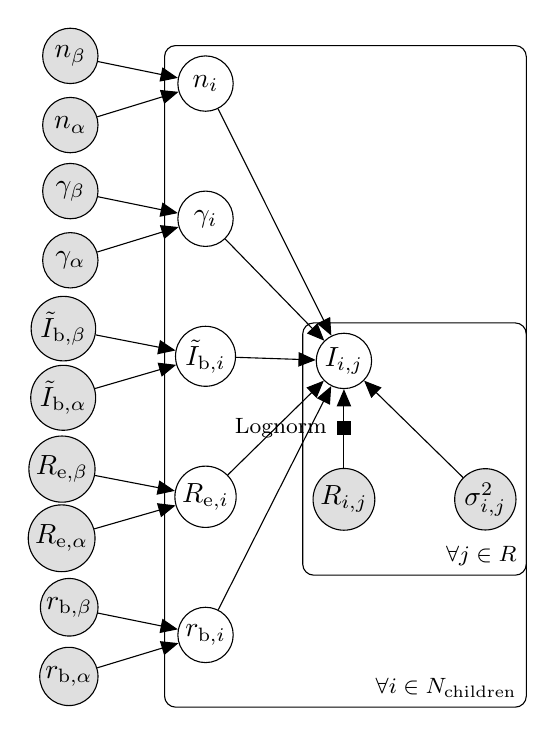
\begin{tikzpicture}
    
    % define nodes
    \node[obs] (r) {$R_{i,j}$};
    \node[obs, right=of r] (sigma) {$\sigma^2_{i,j}$};
    \node[latent, above=of r] (I) {$I_{i,j}$};
    \factor[below=of I] {I-f} {left:Lognorm} {} {};

    \node[latent, left=of r, yshift=-4.9em] (r_b) {$r_{\mathrm{b},i}$};
    \node[latent, above=of r_b] (Re) {$R_{\mathrm{e},i}$};
    \node[latent, above=of Re] (I_b) {$\tilde{I}_{\mathrm{b},i}$};
    \node[latent, above=of I_b] (g) {$\gamma_i$};
    \node[latent, above=of g] (n) {$n_i$};

    \node[obs, left=of r_b, yshift=-1.5em] (r_b_a) {$r_{\mathrm{b},\alpha}$};
    \node[obs, left=of r_b, yshift=1em] (r_b_b) {$r_{\mathrm{b},\beta}$};
    \node[obs, left=of Re, yshift=-1.5em] (Re_a) {$R_{\mathrm{e},\alpha}$};
    \node[obs, left=of Re, yshift=1em] (Re_b) {$R_{\mathrm{e},\beta}$};
    \node[obs, left=of I_b, yshift=-1.5em] (I_b_a) {$\tilde{I}_{\mathrm{b},\alpha}$};
    \node[obs, left=of I_b, yshift=1em] (I_b_b) {$\tilde{I}_{\mathrm{b},\beta}$};
    \node[obs, left=of g, yshift=-1.5em] (g_a) {$\gamma_\alpha$};
    \node[obs, left=of g, yshift=1em] (g_b) {$\gamma_\beta$};
    \node[obs, left=of n, yshift=-1.5em] (n_a) {$n_\alpha$};
    \node[obs, left=of n, yshift=1em] (n_b) {$n_\beta$};


    % connect the nodes
    \edge {r, sigma} {I};

    \edge {r_b, Re, I_b, g, n} {I};

    \edge {r_b_a, r_b_b} {r_b};
    \edge {Re_a, Re_b} {Re};
    \edge {I_b_a, I_b_b} {I_b};
    \edge {g_a, g_b} {g};
    \edge {n_a, n_b} {n};


    % plates
    \plate {rI} {(r)(I)(sigma)} {$\forall j\in R$};
    \plate {pars} {(r)(I)(sigma)(r_b)(Re)(I_b)(g)(n)} {$\forall i\in N_\mathrm{children}$};


\end{tikzpicture}
\end{document}